\documentclass{beamer}
%
% Choose how your presentation looks.
%
% For more themes, color themes and font themes, see:
% http://deic.uab.es/~iblanes/beamer_gallery/index_by_theme.html
%
\mode<presentation>
{
  \usetheme{default}      % or try Darmstadt, Madrid, Warsaw, ...
  \usecolortheme{beaver} % or try albatross, beaver, crane, ...
  \usefonttheme{default}  % or try serif, structurebold, ...
  \setbeamertemplate{navigation symbols}{}
  \setbeamertemplate{caption}[numbered]
} 

\usepackage[english]{babel}
\usepackage[utf8x]{inputenc}
\usepackage{hyperref}
\hypersetup{
    colorlinks=true,
    linkcolor=blue,
    filecolor=magenta,      
    urlcolor=blue,
}

\title[DMI Design]{Introduction to DMI Design}
\author{Andrés Pérez}
\institute{Digital Lutherie\\Master en Música para Experiencias del Entretenimiento\\ENTI-UB}
\date{2018/2019}

\newcommand\blfootnote[1]{%
  \begingroup
  \renewcommand\thefootnote{}\footnote{#1}%
  \addtocounter{footnote}{-1}%
  \endgroup
}

\AtBeginSection[]
{
\begin{frame}{Outline}
    \tableofcontents[currentsection] 
\end{frame}
}

\begin{document}

\begin{frame}
  \titlepage
\end{frame}



\begin{frame}{Outline}
 \tableofcontents
\end{frame}

%%%%%%%%%%%%%%%%%%%%%%%%%%%%%%%%%%%%%%%%%%%%%%%%%%
%%%%%%%%%%%%%%%%%%%%%%%%%%%%%%%%%%%%%%%%%%%%%%%%%%
%%%%%%%%%%%%%%%%%%%%%%%%%%%%%%%%%%%%%%%%%%%%%%%%%%
\section{Introduction}

\begin{frame}{Introduction}
    \textbf{Digital Lutherie}
    \begin{itemize}
        \item Digital: related to computers
        \item Lutherie: musical instrument design and construction
    \end{itemize}
    \vspace{5mm}
    \textbf{DMI: Digital Musical Instrument}
\end{frame}

\begin{frame}{Introduction}
    But... what is a musical instrument?\\
    \vspace{5mm}
    \textit{    "...a music instrument is any device used to play and to produce any music, transforming in real-time (i.e. by being played) the actions of one or more performers into sound events".\footnote{Jordà, S. (2004). Digital Instruments and Players : Part II – Diversity, Freedom and Control, (January 2004).}}
\end{frame}

\begin{frame}{Introduction}
    But... what is a musical instrument?\\
    \vspace{5mm}
    \textit{    "...a music instrument is any device used to play and to produce any music, \textbf{transforming} in real-time (i.e. by being played) the \textbf{actions} of one or more performers into \textbf{sound events}".\footnote{Jordà, S. (2004). Digital Instruments and Players : Part II – Diversity, Freedom and Control, (January 2004).}}
\end{frame}

\begin{frame}{Introduction}
    \begin{figure}[h]
        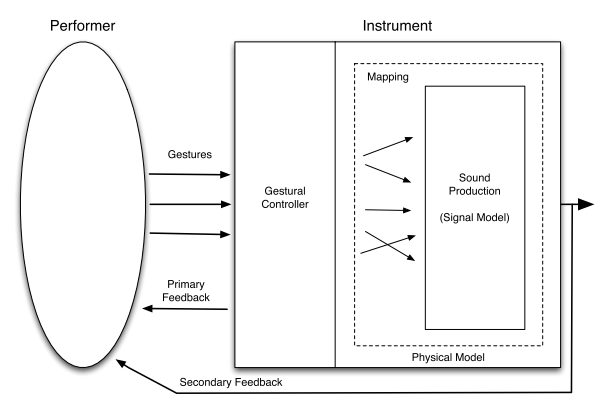
\includegraphics[width=0.9\textwidth]{instrument_scheme.png}\blfootnote{Wanderley, M. M. (2001). Performer-Instrument Interaction: Applications to Gestural Control of Sound Synthesis. PhD thesis, University Paris 6.}
    \end{figure}
\end{frame}

\begin{frame}{Introduction}
    We consider two types of instruments:
    \begin{itemize}
        \item Acoustic (traditional)
        \item Digital
    \end{itemize}
\end{frame}

\begin{frame}{Introduction}
    \textit{    "[...] Perhaps the most fundamental of these differences arises from the separation of the control system from the sound synthesis synthesis in a digital musical instrument (DMI). [...] \textbf{For acoustic instruments these [control systems] are integrated with the sound creation systems}. The performer creates sound on an acoustic instrument by acting directly on the sound production mechanisms"\footnote{Marshall, M. T. (2008). Physical Interface Design for Digital Musical Instruments}.}
\end{frame}

\begin{frame}{Introduction}
    Some consequences for DMI:
    \begin{itemize}
        \item The interface shape (and thus the way of playing the instrument) is not constrained by the sound production method. 
        \item The sound produced by the instrument is not constrained by mechanic/acoustic principles.
        \item The relationship between control system and sound synthesis (\textit{mapping}) is not fixed. 
    \end{itemize}
\end{frame}

\begin{frame}{Introduction}
    In short: DMI design presents a high degree of freedom.\\
    \vspace{5mm}
    So... how should we do???\\
    \vspace{5mm}
    \textit{"... Digital instruments, on their side, are only limited by the imagination and know how of their constructors; a substantial distinction with both positive and negative consequences."\footnote{Jordà, S. (2007). Interactivity and live computer music. Computer Music Journal.}}
\end{frame}



%%%%%%%%%%%%%%%%%%%%%%%%%%%%%%%%%%%%%%%%%%%%%%%%%%
%%%%%%%%%%%%%%%%%%%%%%%%%%%%%%%%%%%%%%%%%%%%%%%%%%
%%%%%%%%%%%%%%%%%%%%%%%%%%%%%%%%%%%%%%%%%%%%%%%%%%
\section{Precursors}

\begin{frame}{Precursors}
    \begin{figure}[h]
        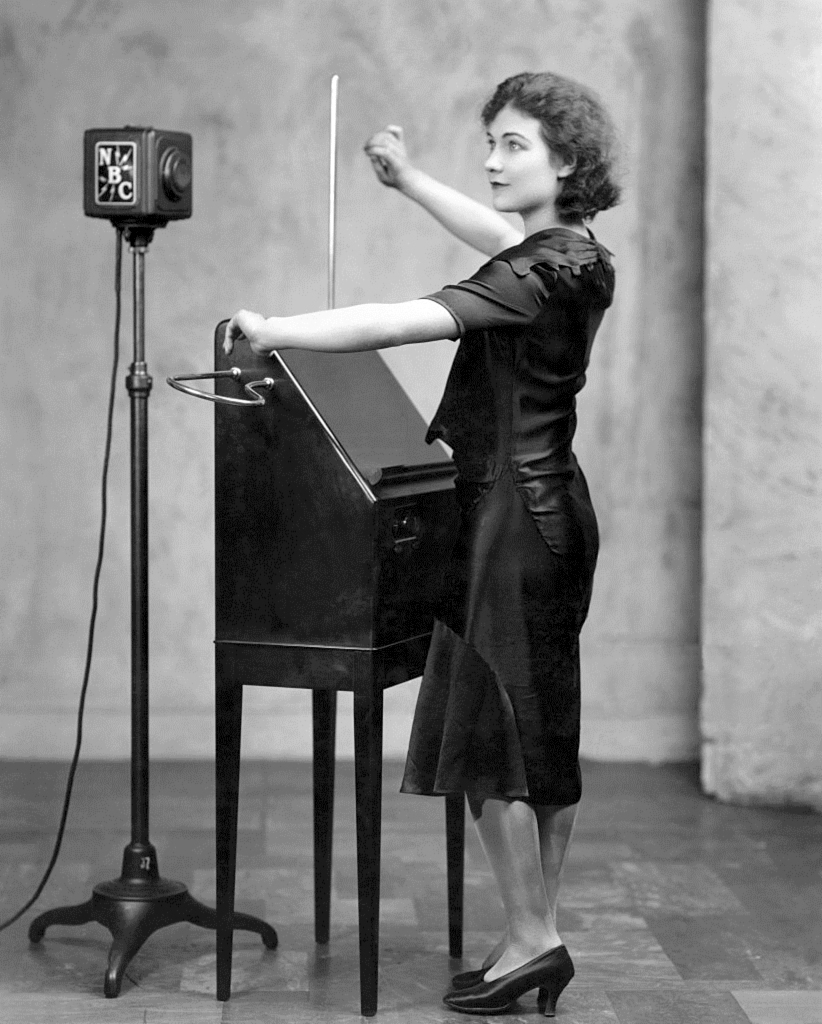
\includegraphics[width=0.5\textwidth]{theremin.jpg}
    \end{figure}
\blfootnote{By What's On the Air Company - What's On the Air, July 1930 (page 45), Public Domain, https://commons.wikimedia.org/w/index.php?curid=56188934}
\end{frame}

\begin{frame}{Precursors}
    \href{https://www.youtube.com/watch?v=uuKBPEDU-W0}{Theremin}
    \vspace{5mm}
    \begin{itemize}
        \item Invented in 1920 by russian engineer Lev Termen 
        \item First successful non-acoustic instrument.
        \item Still commercialized and used nowadays.
        \item Transforms hand gestures into variations of pitch and volume.
        \item Based on electric resonators and the heterodyne principle.
    \end{itemize}
\end{frame}

\begin{frame}{Precursors}
    \begin{figure}[h]
        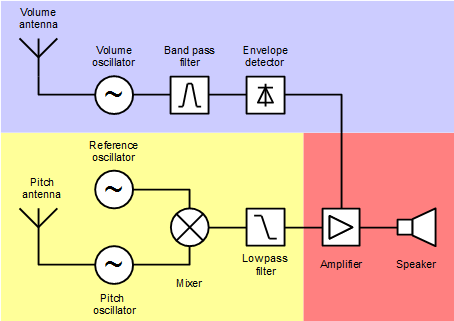
\includegraphics[width=0.8\textwidth]{theremin_scheme.png}
    \end{figure}
\blfootnote{By DF5GO - Own work, CC BY-SA 3.0, https://commons.wikimedia.org/w/index.php?curid=30234604}
\end{frame}

\begin{frame}{Precursors}
    \begin{figure}[h]
        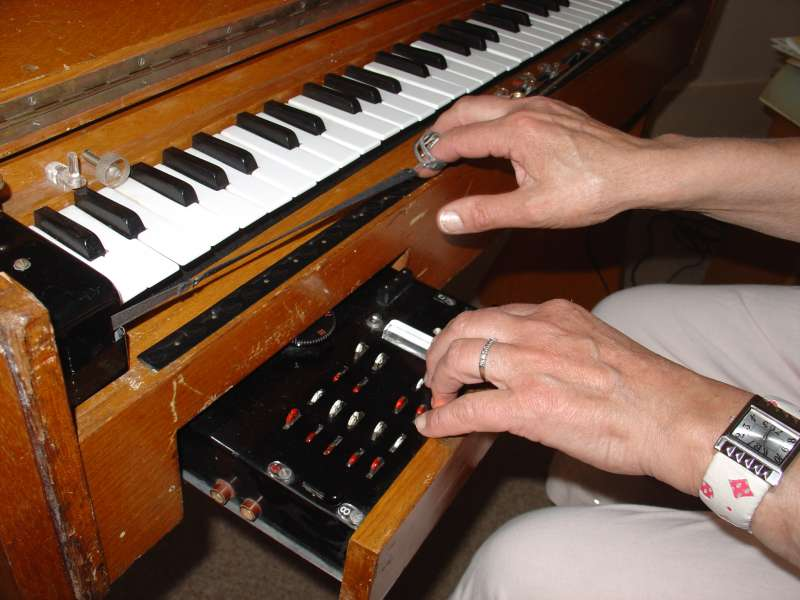
\includegraphics[width=0.8\textwidth]{ondes.jpg}
    \end{figure}
\blfootnote{By User:30rKs56MaE - Own work, CC BY-SA 3.0, https://commons.wikimedia.org/w/index.php?curid=19804023}
\end{frame}

\begin{frame}{Precursors}
    \href{https://www.youtube.com/watch?v=v0aflcF0-ys}{Ondes Martenot}
    \vspace{5mm}
    \begin{itemize}
        \item Invented in 1928 by frech cellist Maurice Martenot
        \item Electrical synthesizer.
        \item Pitch is controlled by right hand, volume and timbre with left hand.
        \item Popularized by Radiohead in the 2000's.
    \end{itemize}
\end{frame}

\begin{frame}{Precursors}
    \begin{figure}[h]
        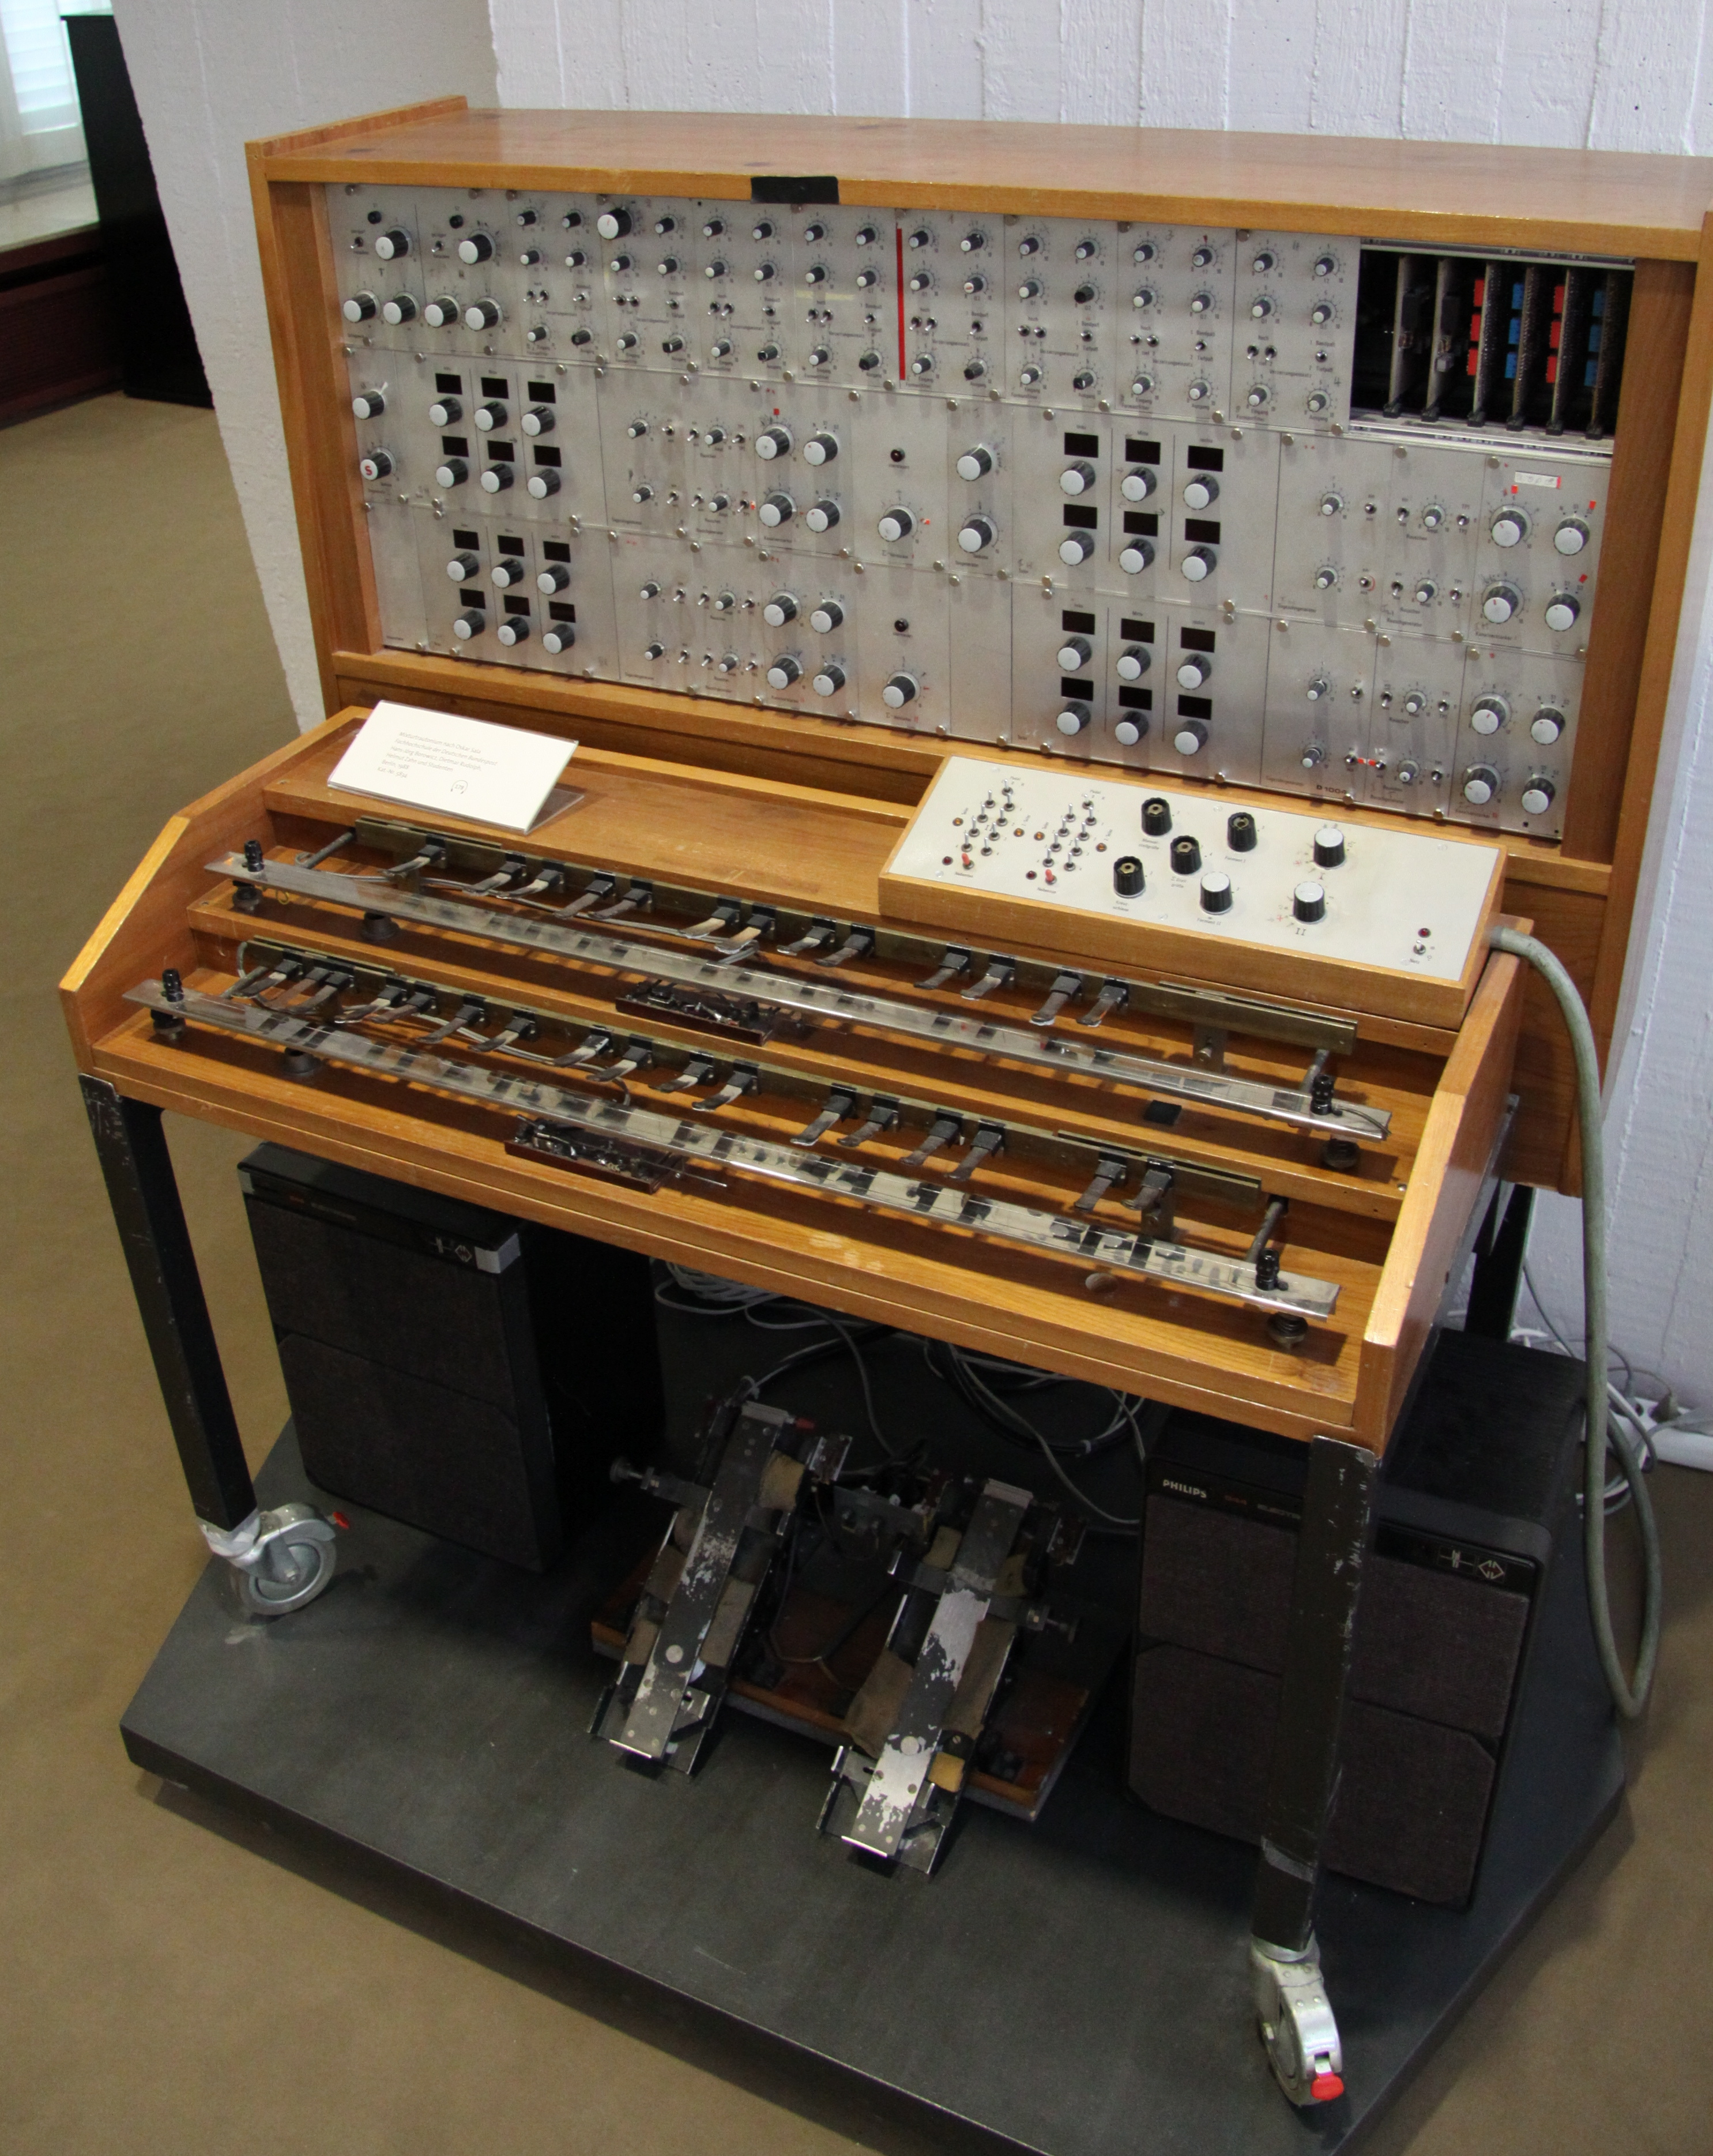
\includegraphics[width=0.5\textwidth]{trautonium.jpg}
    \end{figure}
\blfootnote{By Morn the Gorn - Own work, CC BY-SA 3.0, https://commons.wikimedia.org/w/index.php?curid=9782324}
\end{frame}

\begin{frame}{Precursors}
    \href{https://www.youtube.com/watch?v=uaWrdbvhg1Q}{Trautonium}
    \vspace{5mm}
    \begin{itemize}
        \item Invented in 1929 by german electrical engineer Friedrich Trautwein.
        \item Player gestures change resistivity of a metal plate, trasforming into pitch and volume changes.
        \item Extensely played and improved by Oskar Sala (Mixturtrautonium).
        \item Innovative introduction of formant filters for timbral control.
    \end{itemize}
\end{frame}

\begin{frame}{Precursors}
    \begin{figure}[h]
        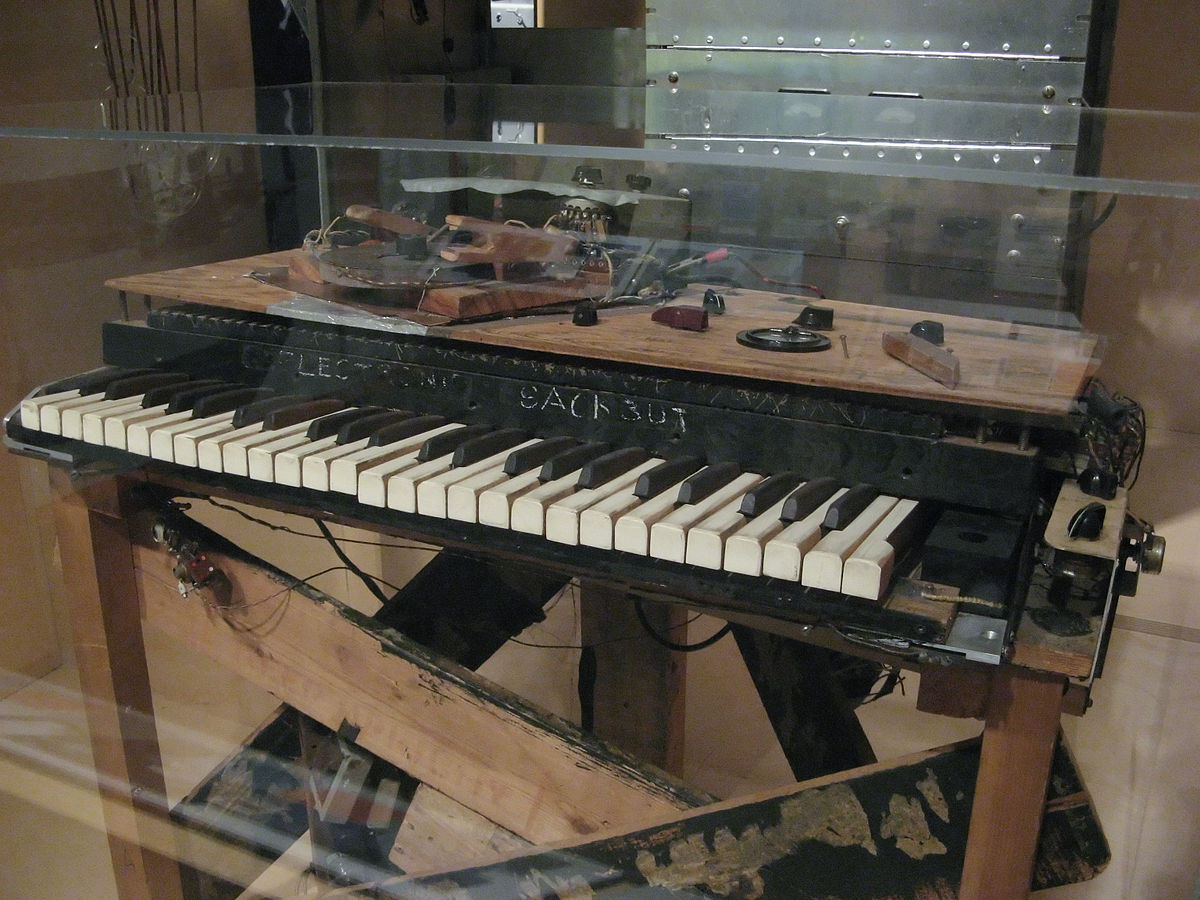
\includegraphics[width=0.8\textwidth]{sackbut.jpg}
    \end{figure}
\blfootnote{By David Carroll - originally posted to Flickr as image0243, CC BY 2.0, https://commons.wikimedia.org/w/index.php?curid=7531112}
\end{frame}

\begin{frame}{Precursors}
    \href{https://www.youtube.com/watch?v=yfpKj5KpneA}{Electronic Sackbut}
    \vspace{5mm}
    \begin{itemize}
        \item Invented in 1945 by canadian physicist Hugh Le Caine.
        \item Predecessor of voltage-controlled synths
        \item 2D continuous control of volume, attack and pitch
    \end{itemize}
\end{frame}

\begin{frame}{Precursors}
    Some thoughts...
    \vspace{5mm}
    \begin{itemize}
        \item All instrument designers were primarily scientists!
        \item Huge bias towards "improving the piano"
        \item Huge bias towards continuous (pitch) control
        \item These are not exactly DMIs...
    \end{itemize}
    \vspace{5mm}
    Many other bizarre creations at \href{http://120years.net/}{120 Years of Electronic Music}
\end{frame}


\end{document}
